% Options for packages loaded elsewhere
\PassOptionsToPackage{unicode}{hyperref}
\PassOptionsToPackage{hyphens}{url}
%
\documentclass[
]{article}
\usepackage{amsmath,amssymb}
\usepackage{iftex}
\ifPDFTeX
  \usepackage[T1]{fontenc}
  \usepackage[utf8]{inputenc}
  \usepackage{textcomp} % provide euro and other symbols
\else % if luatex or xetex
  \usepackage{unicode-math} % this also loads fontspec
  \defaultfontfeatures{Scale=MatchLowercase}
  \defaultfontfeatures[\rmfamily]{Ligatures=TeX,Scale=1}
\fi
\usepackage{lmodern}
\ifPDFTeX\else
  % xetex/luatex font selection
\fi
% Use upquote if available, for straight quotes in verbatim environments
\IfFileExists{upquote.sty}{\usepackage{upquote}}{}
\IfFileExists{microtype.sty}{% use microtype if available
  \usepackage[]{microtype}
  \UseMicrotypeSet[protrusion]{basicmath} % disable protrusion for tt fonts
}{}
\makeatletter
\@ifundefined{KOMAClassName}{% if non-KOMA class
  \IfFileExists{parskip.sty}{%
    \usepackage{parskip}
  }{% else
    \setlength{\parindent}{0pt}
    \setlength{\parskip}{6pt plus 2pt minus 1pt}}
}{% if KOMA class
  \KOMAoptions{parskip=half}}
\makeatother
\usepackage{xcolor}
\usepackage[margin=1in]{geometry}
\usepackage{color}
\usepackage{fancyvrb}
\newcommand{\VerbBar}{|}
\newcommand{\VERB}{\Verb[commandchars=\\\{\}]}
\DefineVerbatimEnvironment{Highlighting}{Verbatim}{commandchars=\\\{\}}
% Add ',fontsize=\small' for more characters per line
\usepackage{framed}
\definecolor{shadecolor}{RGB}{248,248,248}
\newenvironment{Shaded}{\begin{snugshade}}{\end{snugshade}}
\newcommand{\AlertTok}[1]{\textcolor[rgb]{0.94,0.16,0.16}{#1}}
\newcommand{\AnnotationTok}[1]{\textcolor[rgb]{0.56,0.35,0.01}{\textbf{\textit{#1}}}}
\newcommand{\AttributeTok}[1]{\textcolor[rgb]{0.13,0.29,0.53}{#1}}
\newcommand{\BaseNTok}[1]{\textcolor[rgb]{0.00,0.00,0.81}{#1}}
\newcommand{\BuiltInTok}[1]{#1}
\newcommand{\CharTok}[1]{\textcolor[rgb]{0.31,0.60,0.02}{#1}}
\newcommand{\CommentTok}[1]{\textcolor[rgb]{0.56,0.35,0.01}{\textit{#1}}}
\newcommand{\CommentVarTok}[1]{\textcolor[rgb]{0.56,0.35,0.01}{\textbf{\textit{#1}}}}
\newcommand{\ConstantTok}[1]{\textcolor[rgb]{0.56,0.35,0.01}{#1}}
\newcommand{\ControlFlowTok}[1]{\textcolor[rgb]{0.13,0.29,0.53}{\textbf{#1}}}
\newcommand{\DataTypeTok}[1]{\textcolor[rgb]{0.13,0.29,0.53}{#1}}
\newcommand{\DecValTok}[1]{\textcolor[rgb]{0.00,0.00,0.81}{#1}}
\newcommand{\DocumentationTok}[1]{\textcolor[rgb]{0.56,0.35,0.01}{\textbf{\textit{#1}}}}
\newcommand{\ErrorTok}[1]{\textcolor[rgb]{0.64,0.00,0.00}{\textbf{#1}}}
\newcommand{\ExtensionTok}[1]{#1}
\newcommand{\FloatTok}[1]{\textcolor[rgb]{0.00,0.00,0.81}{#1}}
\newcommand{\FunctionTok}[1]{\textcolor[rgb]{0.13,0.29,0.53}{\textbf{#1}}}
\newcommand{\ImportTok}[1]{#1}
\newcommand{\InformationTok}[1]{\textcolor[rgb]{0.56,0.35,0.01}{\textbf{\textit{#1}}}}
\newcommand{\KeywordTok}[1]{\textcolor[rgb]{0.13,0.29,0.53}{\textbf{#1}}}
\newcommand{\NormalTok}[1]{#1}
\newcommand{\OperatorTok}[1]{\textcolor[rgb]{0.81,0.36,0.00}{\textbf{#1}}}
\newcommand{\OtherTok}[1]{\textcolor[rgb]{0.56,0.35,0.01}{#1}}
\newcommand{\PreprocessorTok}[1]{\textcolor[rgb]{0.56,0.35,0.01}{\textit{#1}}}
\newcommand{\RegionMarkerTok}[1]{#1}
\newcommand{\SpecialCharTok}[1]{\textcolor[rgb]{0.81,0.36,0.00}{\textbf{#1}}}
\newcommand{\SpecialStringTok}[1]{\textcolor[rgb]{0.31,0.60,0.02}{#1}}
\newcommand{\StringTok}[1]{\textcolor[rgb]{0.31,0.60,0.02}{#1}}
\newcommand{\VariableTok}[1]{\textcolor[rgb]{0.00,0.00,0.00}{#1}}
\newcommand{\VerbatimStringTok}[1]{\textcolor[rgb]{0.31,0.60,0.02}{#1}}
\newcommand{\WarningTok}[1]{\textcolor[rgb]{0.56,0.35,0.01}{\textbf{\textit{#1}}}}
\usepackage{longtable,booktabs,array}
\usepackage{calc} % for calculating minipage widths
% Correct order of tables after \paragraph or \subparagraph
\usepackage{etoolbox}
\makeatletter
\patchcmd\longtable{\par}{\if@noskipsec\mbox{}\fi\par}{}{}
\makeatother
% Allow footnotes in longtable head/foot
\IfFileExists{footnotehyper.sty}{\usepackage{footnotehyper}}{\usepackage{footnote}}
\makesavenoteenv{longtable}
\usepackage{graphicx}
\makeatletter
\def\maxwidth{\ifdim\Gin@nat@width>\linewidth\linewidth\else\Gin@nat@width\fi}
\def\maxheight{\ifdim\Gin@nat@height>\textheight\textheight\else\Gin@nat@height\fi}
\makeatother
% Scale images if necessary, so that they will not overflow the page
% margins by default, and it is still possible to overwrite the defaults
% using explicit options in \includegraphics[width, height, ...]{}
\setkeys{Gin}{width=\maxwidth,height=\maxheight,keepaspectratio}
% Set default figure placement to htbp
\makeatletter
\def\fps@figure{htbp}
\makeatother
\ifLuaTeX
  \usepackage{luacolor}
  \usepackage[soul]{lua-ul}
\else
  \usepackage{soul}
\fi
\setlength{\emergencystretch}{3em} % prevent overfull lines
\providecommand{\tightlist}{%
  \setlength{\itemsep}{0pt}\setlength{\parskip}{0pt}}
\setcounter{secnumdepth}{-\maxdimen} % remove section numbering
% definitions for citeproc citations
\NewDocumentCommand\citeproctext{}{}
\NewDocumentCommand\citeproc{mm}{%
  \begingroup\def\citeproctext{#2}\cite{#1}\endgroup}
\makeatletter
 % allow citations to break across lines
 \let\@cite@ofmt\@firstofone
 % avoid brackets around text for \cite:
 \def\@biblabel#1{}
 \def\@cite#1#2{{#1\if@tempswa , #2\fi}}
\makeatother
\newlength{\cslhangindent}
\setlength{\cslhangindent}{1.5em}
\newlength{\csllabelwidth}
\setlength{\csllabelwidth}{3em}
\newenvironment{CSLReferences}[2] % #1 hanging-indent, #2 entry-spacing
 {\begin{list}{}{%
  \setlength{\itemindent}{0pt}
  \setlength{\leftmargin}{0pt}
  \setlength{\parsep}{0pt}
  % turn on hanging indent if param 1 is 1
  \ifodd #1
   \setlength{\leftmargin}{\cslhangindent}
   \setlength{\itemindent}{-1\cslhangindent}
  \fi
  % set entry spacing
  \setlength{\itemsep}{#2\baselineskip}}}
 {\end{list}}
\usepackage{calc}
\newcommand{\CSLBlock}[1]{\hfill\break\parbox[t]{\linewidth}{\strut\ignorespaces#1\strut}}
\newcommand{\CSLLeftMargin}[1]{\parbox[t]{\csllabelwidth}{\strut#1\strut}}
\newcommand{\CSLRightInline}[1]{\parbox[t]{\linewidth - \csllabelwidth}{\strut#1\strut}}
\newcommand{\CSLIndent}[1]{\hspace{\cslhangindent}#1}
\ifLuaTeX
  \usepackage{selnolig}  % disable illegal ligatures
\fi
\usepackage{bookmark}
\IfFileExists{xurl.sty}{\usepackage{xurl}}{} % add URL line breaks if available
\urlstyle{same}
\hypersetup{
  pdftitle={\{censobr\}: Easy Access to Brazilian Population Census Data},
  pdfauthor={Rafael H. M. Pereira, IPEA; Rogério Jerônimo Barbosa, IESP/UERJ},
  hidelinks,
  pdfcreator={LaTeX via pandoc}}

\title{\texttt{\{censobr\}}: Easy Access to Brazilian Population Census
Data}
\author{Rafael H. M. Pereira, IPEA \and Rogério Jerônimo Barbosa,
IESP/UERJ}
\date{2024-11-21}

\begin{document}
\maketitle

\subsection{1. Introduction}\label{introduction}

Population census data is one of the most important sources of
information on the characteristics and living conditions of populations.
In Brazil, the population census conducted by the Brazilian Institute of
Geography and Statistics (IBGE) is an essential resource for scientific
research and serves as a cornerstone for informing government policies
and planning. However, the raw data format of Brazilian census data
released to the public and the large size of these data sets often poses
substantial challenges for researchers, particularly those working with
limited computing resources.

To address these issues, we developed \texttt{\{censobr\}}, an R package
designed to facilitate the efficient access and manipulation of
Brazilian census data and documentation, covering all editions of the
census since 1960. Because the \texttt{\{censobr\}} package builds on
the Apache Arrow platform and preprocessed files saved in
\texttt{.parquet} format, it enables users to manage larger-than-memory
datasets using a columnar memory format that optimizes data access and
processing. Arrow seamlessly integrates with \texttt{\{dplyr\}} syntax,
allowing users to interact with in-disk datasets using familiar R
commands, thus streamlining the analytical workflow without
necessitating extensive new learning. \texttt{\{censobr\}} also
integrates with \texttt{\{geobr\}} (Pereira and Goncalves 2019), an R
package to download official geospatial data in Brazil, using matching
geographic identifiers that facilitate the merging of census data with
spatial geometries for visualization and analysis. Our goal is to make
census data more accessible while maintaining the flexibility and power
of the R environment.

This paper introduces the \texttt{\{censobr\}} package, outlines its
core functionalities, and provides illustrative examples that
demonstrate its applications in social science research.

\subsection{2. An Overview of Brazilian Population
Censuses}\label{an-overview-of-brazilian-population-censuses}

The first census of Brazil was conducted in 1872, during Brazil's
imperial period, while modern censuses began in 1940 under the
coordination of the Brazilian Institute of Geography and Statistics
(IBGE) (IBGE 1990). Given the size of the country in terms of both
population and territory, the Brazilian population census represents one
of the most extensive population data collection initiatives worldwide.

Since 1960, each Brazilian census is divided into two main components:
the \textbf{universe survey} and the \textbf{sample survey} (similar to
census data collection in other countries like the United States and
\ldots.. ). The universal survey is administered to all households and
collects essential demographic and housing information through a short
questionnaire containing between 9 and 30 questions, depending on the
census edition. In contrast, the sample survey targets a representative
subset of the population and uses a longer questionnaire that includes
all questions from the universe components as well as dozens of more
detailed questions on topics such as migration, religion, education,
fertility, income, and employment. The sample size was 25\% in the 1960,
1970, and 1980 censuses, and it was reduced to 10\% from 1991 onwards
(REF).

Brazilian population census data is published in two main formats:
aggregated data at the census tract level, and microdata at the person
or household level. \textbf{Aggregated data} from the universe survey
(short questionnaire) provide summary statistics (counts, proportions,
and means) computed at the census tract level. This data set can be used
for example for spatial analysis to examine spatial patterns,
disparities and trends of various characteristics of the population
(e.g. Brueckner, Mation, and Nadalin 2019; Goto, Suarez, and Ye 2022).
\textbf{Census tracts} are the smallest geographic unit in the censuses.
They are contiguous areas typically containing about 200 households,
designed to facilitate efficient enumeration and data collection. Over
time, the number of census tracts has expanded in response to population
growth and changes in settlement patterns, with approximately 216,000
census tracts in 2000, 314,000 in 2010, and 452,000 in 2022. These
tracts form the fundamental spatial units for census data collection,
reflecting the evolution of Brazilian urban and rural landscapes.
Individual-level data from the universe survey is not publicly available
due to privacy concerns.

Meanwhile, the \textbf{microdata} from the sample survey (long
questionnaire) consist of a dataset in which each row represents an
instance of data collection. In IBGE surveys and censuses, ``persons''
and ``households'' are tipically the units of analysis of microdata.
``Persons'' refer to individual members of the population, and their
data typically includes personal characteristics such as age, gender,
education, etc. ``Households'' represent residential units, which
consist of one or more persons living together, sharing living expenses,
and typically occupying a single housing unit. Household-level microdata
include variables related to housing conditions, access to services
(such as water and sanitation) and household composition (such as the
number of residents and their relationships). Because the sample survey
is more sparse geographically, it does not allow for fine-grained
spatial analyses. The smallest geographic units available in the
microdata are \textbf{weighting areas} (áreas de ponderação), which are
groups of contiguous census tracts ensuring statistical
representativeness. For the 2010 Census, IBGE established that a
weighting area should have at least 400 occupied households in the
sample. In less densely populated regions, these areas cover a large
territorial extension.

In summary, there is a trade-off of spatial granularity and richness of
information between the the universe and the sample survey components of
the Brazilian census. While aggregated data at the census tract level
allows for fine grained spatial, it covers relatively few variables. By
contrast, the microdata from the sample survey covers many more
variables that allow for detailed individual- and household-level
analysis, but at a coarser geographical level.

6666666666666666666666666666 \st{By using \textbf{sampling weights}
included in the sample microdata, users can generate population
estimates that accurately reflect the Brazilian entire population. As
the sample was not produced using Simple Random Sampling (SRS),
statistical inference requires accounting for the complex sampling
design used in the census, which affects variance estimates and
confidence interval calculations.}

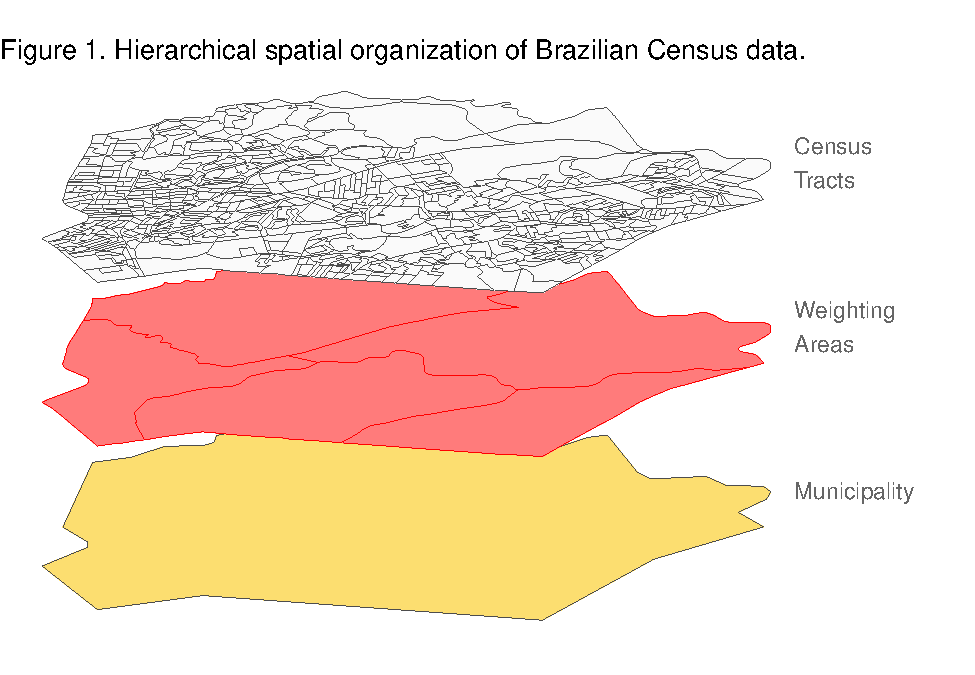
\includegraphics{C:/1_Artigos/censobr_paper_2025/paper_pdf/censobr_shortPaper_files/figure-latex/unnamed-chunk-1-1.pdf}

\subsection{3. Installation and Core Data
Functions}\label{installation-and-core-data-functions}

\texttt{\{censobr\}} is available on CRAN, and the stable version can be
installed like any other R package using the \texttt{install.packages()}
function:

\begin{Shaded}
\begin{Highlighting}[]
\FunctionTok{install.packages}\NormalTok{(}\StringTok{"censobr"}\NormalTok{)}
\end{Highlighting}
\end{Shaded}

Users interested in accessing the latest features can install the
development version directly from GitHub using:

\begin{Shaded}
\begin{Highlighting}[]
\CommentTok{\# First, remove any existing version of censobr}
\NormalTok{utils}\SpecialCharTok{::}\FunctionTok{remove.packages}\NormalTok{(}\StringTok{"censobr"}\NormalTok{)}

\CommentTok{\# Install the development version from GitHub}
\NormalTok{remotes}\SpecialCharTok{::}\FunctionTok{install\_github}\NormalTok{(}\StringTok{"ipeaGIT/censobr"}\NormalTok{, }\AttributeTok{ref =} \StringTok{"dev"}\NormalTok{)}
\end{Highlighting}
\end{Shaded}

After installing \texttt{\{censobr\}}, load it into your R session with:

\begin{Shaded}
\begin{Highlighting}[]
\FunctionTok{library}\NormalTok{(censobr)}
\end{Highlighting}
\end{Shaded}

The package includes several core functions to download and read
different types of census data:

\textbf{Table 1. Core data functions in the \{censobr\} package.}

\begin{longtable}[]{@{}
  >{\raggedright\arraybackslash}p{(\columnwidth - 4\tabcolsep) * \real{0.2564}}
  >{\raggedright\arraybackslash}p{(\columnwidth - 4\tabcolsep) * \real{0.5641}}
  >{\raggedright\arraybackslash}p{(\columnwidth - 4\tabcolsep) * \real{0.1795}}@{}}
\toprule\noalign{}
\begin{minipage}[b]{\linewidth}\raggedright
Function
\end{minipage} & \begin{minipage}[b]{\linewidth}\raggedright
Description
\end{minipage} & \begin{minipage}[b]{\linewidth}\raggedright
Availability
\end{minipage} \\
\midrule\noalign{}
\endhead
\bottomrule\noalign{}
\endlastfoot
\texttt{read\_population()} & Download microdata of population records &
1960, 1970, 1980, 1991, 2000, 2010 (\emph{soon} for 2022) \\
& & \\
\texttt{read\_households()} & Download microdata of household records &
1960, 1970, 1980, 1991, 2000, 2010 (\emph{soon} for 2022) \\
& & \\
\texttt{read\_mortality()} & Download microdata of death records & 2010
(\emph{soon} for 2022) \\
& & \\
\texttt{read\_emigration()} & Download microdata of emigration records &
2010 (\emph{soon} for 2022) \\
& & \\
\texttt{read\_families()} & Download microdata of family records &
2000 \\
& & \\
\texttt{read\_tracts()} & Download census tract-level aggregated data &
2010 (\emph{soon} for 2000 and 2022) \\
\end{longtable}

These functions allow users to specify the year and type of data they
want to access, and whether the function should return the data in a
format compatible with Arrow or a regular \texttt{data.frame} (see next
section). The first time the user runs a function, \texttt{\{censobr\}}
will download the data file in \texttt{.parquet} format and store it
locally. This way, the data only needs to be downloaded once (more info
on section 7).

All data sets available through \texttt{\{censobr\}} are identical to
data published by IBGE, the only difference being that the data sets in
\texttt{\{censobr\}} are enriched with geography columns following the
name standards of the \texttt{\{geobr\}} package to facilitate
integration with spatial data. The only exception to this is the data
from the 1960 census, which is the result of a careful data process to
rebuild the original data, as detailed below.

\subsubsection{3.1 The 1960 census}\label{the-1960-census}

The microdata version available in \texttt{\{censobr\}} represents a
combination of two distinct datasets drawn from the 1960 population
census. The 1960 Census in Brazil marked a significant chapter in the
nation's demographic data collection history, characterized by both
methodological complexity and subsequent challenges in data processing.
Initially, IBGE conducted a comprehensive 25\% sample survey alongside
the universe census, but technical issues delayed its processing, and
several states' data remained incomplete and undigitized. The 25\%
sample currently available includes only 16 states of the Federation,
excluding Maranhão, Piauí, Guanabara, Santa Catarina, Espírito Santo,
and the Northern Region. It also contains data from a contested border
region between Minas Gerais and Espírito Santo known as Serra dos
Aimorés.

In the midst of the processing delay, in 1965, IBGE also created a
probabilistic sub-sample representing approximately 1.27\% of the
population, covering all units of the Federation. This sub-sample was
used to produce several official reports in the 1960s, and it remains an
important source of data. Unlike the 25\% sample, the 1.27\% dataset is
comprehensive in terms of geographic coverage, encompassing states not
included in the 25\% sample (which was never fully processed), albeit
excluding rural areas of the state of Rondônia. We combined both the
25\% and 1.27\% samples to form a more complete dataset, which
approximates the original design intended for the 1960 Census. The
merging process involved substantial pre-processing to address data
inconsistencies, especially since portions of the original 1.27\% sample
were corrupted, leading to missing or inaccurate information. A detailed
explanation of how these data was processed is available at
\url{https://github.com/antrologos/ConsistenciaCenso1960Br}.

We development a crosswalk to align municipality codes from the 1960
Census with municipality names, using auxiliary documents from the
IBGE's online library, with extensive manual digitization required due
to the low quality of the scanned documents. Using the municipality
names, we matched 1960 Census with the Brazilian Statistical Yearbook
(Anuário Estatístico Brasileiro) and imported detailed information on
the population totals of rural and urban areas for all municipalities
and states. This allowed us to construct a sample weight variable,
enabling proper population estimates and correcting for unbalanced data.
For the 25\% sample observations, the weights expand to the municipal
level, while for the 1.27\% sample observations, the expansion occurs at
the state level. Additionally, to approximate the original complex
sample design and allow for more accurate statistical analysis,
variables representing stratification and clustering were incorporated.
This feature enables the calculation of standard errors and confidence
intervals that properly account for the combined sampling structure.

We believe the availability of these combined datasets of the 1960
Census in the \texttt{\{censobr\}} package offers a unique opportunity
for researchers interested in studying Brazil's demographic history
during a period marked by rapid urbanization and socioeconomic
transformation.

\subsection{\texorpdfstring{4. Census Documentation Available in
\texttt{\{censobr\}}}{4. Census Documentation Available in \{censobr\}}}\label{census-documentation-available-in-censobr}

In addition to functions for data reading, the \texttt{\{censobr\}}
package also provides a set of functions for quick access to census
documentation, including variable dictionaries, questionnaires, and
interviewer manuals.

\textbf{Table 2. Documentation functions in the \{censobr\} package.}

\begin{longtable}[]{@{}
  >{\raggedright\arraybackslash}p{(\columnwidth - 4\tabcolsep) * \real{0.2121}}
  >{\raggedright\arraybackslash}p{(\columnwidth - 4\tabcolsep) * \real{0.2222}}
  >{\raggedright\arraybackslash}p{(\columnwidth - 4\tabcolsep) * \real{0.5657}}@{}}
\toprule\noalign{}
\begin{minipage}[b]{\linewidth}\raggedright
Function
\end{minipage} & \begin{minipage}[b]{\linewidth}\raggedright
Description
\end{minipage} & \begin{minipage}[b]{\linewidth}\raggedright
Availability
\end{minipage} \\
\midrule\noalign{}
\endhead
\bottomrule\noalign{}
\endlastfoot
\texttt{data\_dictionary()} & Download data dictionary (code book) &
Microdata: 1960, 1970, 1980, 1991, 2000, 2010 (\emph{soon} for 2022) \\
& & \\
& & Tract-level aggregates: 2000, 2010 (\emph{soon} for 2022) \\
& & \\
& & \\
\texttt{questionnaire()} & Download questionnaires used in data
collection & 1960, 1970, 1980, 1991, 2000, 2010, 2022 \\
& & \\
\texttt{interview\_manual()} & Download interview manual (guidebook) for
surveyors & 1960, 1970, 1980, 1991, 2000, 2010, 2022 \\
\end{longtable}

All documentation functions download the files in \texttt{.html} or
\texttt{.pdf} format and open the document in the browser. Similar to
the data reading functions of \texttt{\{censobr\}}, these documentation
functions also save the files in a local cache the first time the
function is run. Thus, when the user runs the function again, the
package simply loads the local file almost instantly.

\subsubsection{4.1. Data Dictionary}\label{data-dictionary}

The \texttt{data\_dictionary()} function loads the variable dictionary,
pointing to the definition of each variable and the meaning of its
categories for categorical variables. Currently, the function covers the
sample microdata dictionaries for all Brazilian censuses since 1960:
\texttt{c(1960,\ 1970,\ 1980,\ 1991,\ 2000,\ and\ 2010)}. Additionally,
the function also includes the dictionaries for census tract-level
aggregate data for the years 2000 and 2010.

\begin{Shaded}
\begin{Highlighting}[]
\CommentTok{\# dictionary of variables: population microdata}
\FunctionTok{data\_dictionary}\NormalTok{(}\AttributeTok{year =} \DecValTok{2010}\NormalTok{, }
                \AttributeTok{dataset =} \StringTok{\textquotesingle{}population\textquotesingle{}}\NormalTok{)}

\CommentTok{\# dictionary of variables: household microdata}
\FunctionTok{data\_dictionary}\NormalTok{(}\AttributeTok{year =} \DecValTok{2010}\NormalTok{, }
                \AttributeTok{dataset =} \StringTok{\textquotesingle{}households\textquotesingle{}}\NormalTok{)}

\CommentTok{\# dictionary of census tract variables (aggregate data)}
\FunctionTok{data\_dictionary}\NormalTok{(}\AttributeTok{year =} \DecValTok{2010}\NormalTok{, }
                \AttributeTok{dataset =} \StringTok{\textquotesingle{}tracts\textquotesingle{}}\NormalTok{)}
\end{Highlighting}
\end{Shaded}

\subsubsection{4.2. Questionnaires}\label{questionnaires}

Understanding the structure and flow of a questionnaire is often crucial
for effective data analysis. The \texttt{questionnaire()} function
includes the questionnaires used in data collection for all Brazilian
censuses since 1960. In addition to passing the \texttt{year} parameter,
the user needs to indicate the type of questionnaire of interest,
whether it is the short form for the universe survey
(\texttt{type\ =\ \textquotesingle{}short\textquotesingle{}}) or the
long form used in the sample survey
(\texttt{type\ =\ \textquotesingle{}long\textquotesingle{}}).

\begin{Shaded}
\begin{Highlighting}[]
\CommentTok{\# short questionnaire for the universe survey}
\FunctionTok{questionnaire}\NormalTok{(}\AttributeTok{year =} \DecValTok{2022}\NormalTok{, }
              \AttributeTok{type =} \StringTok{\textquotesingle{}short\textquotesingle{}}\NormalTok{)}

\CommentTok{\# long questionnaire for the sample survey}
\FunctionTok{questionnaire}\NormalTok{(}\AttributeTok{year =} \DecValTok{2022}\NormalTok{, }
              \AttributeTok{type =} \StringTok{\textquotesingle{}long\textquotesingle{}}\NormalTok{)}
\end{Highlighting}
\end{Shaded}

\subsubsection{4.3. Interviewer Manual}\label{interviewer-manual}

Finally, the \texttt{interview\_manual()} function downloads and opens
in the browser the ``Manual do Recenseador,'' i.e., the instruction
manual for IBGE enumerators on how to collect census data. Manuals for
all censuses since 1960 are available.

\begin{Shaded}
\begin{Highlighting}[]
\CommentTok{\# 2022 Census}
\FunctionTok{interview\_manual}\NormalTok{(}\AttributeTok{year =} \DecValTok{2022}\NormalTok{)}

\CommentTok{\# 1960 Census}
\FunctionTok{interview\_manual}\NormalTok{(}\AttributeTok{year =} \DecValTok{1960}\NormalTok{)}
\end{Highlighting}
\end{Shaded}

\subsection{5. Handling Larger-Than-Memory
Data}\label{handling-larger-than-memory-data}

\subsubsection{\texorpdfstring{5.1. In-disk Data wrangling with
\texttt{\{arrow\}} and working with databases with \texttt{\{duckdb\}}
and
\texttt{\{dbplyr\}}}{5.1. In-disk Data wrangling with \{arrow\} and working with databases with \{duckdb\} and \{dbplyr\}}}\label{in-disk-data-wrangling-with-arrow-and-working-with-databases-with-duckdb-and-dbplyr}

One of the most essential features of \texttt{\{censobr\}} is its
capability to handle larger-than-memory datasets. The Brazilian census
datasets are often too large to load directly into users' RAM. To
address this, \texttt{\{censobr\}} uses files saved in \texttt{.parquet}
format, and by default, returns an ``Arrow table'' rather than a
conventional \texttt{data.frame}. An Arrow table is an object that
points to the dataset stored on disk, allowing for basic data
manipulation without loading it into memory entirely.

Once the desired data are accessed through any \texttt{read\_*}
function, users can use common \texttt{\{dplyr\}} functions to select
columns, filter cases, recode variables, or aggregate observations.
Operations on Arrow tables are executed lazily; that is, they are only
evaluated when explicitly requested, allowing researchers to delay heavy
computations until they are necessary. After processing, smaller, more
manageable datasets can be collected for further analysis.

To retrieve the results, users have two options:

\begin{itemize}
\tightlist
\item
  \textbf{\texttt{collect()}}: Converts the results into a regular
  \texttt{data.frame} loaded on the RAM memory.
\item
  \textbf{\texttt{compute()}}: Materializes the results as a new Arrow
  table, keeping it in Arrow format.
\end{itemize}

In this quick example below, we read the data with all the 111.555
observations of deaths recorded in the 2010 census, but this data is not
loaded to the RAM memory. Once we filter the data to keep only the
deaths of men in the state of Rio de Janeiro (RJ), it is only after we
perform the \texttt{collect()} tha the result is loaded to memory as a
\texttt{data.frame} with 3.947 observations.

\begin{Shaded}
\begin{Highlighting}[]
\CommentTok{\# Read 2010 mortality data}
\NormalTok{mortality\_2010 }\OtherTok{\textless{}{-}}\NormalTok{ censobr}\SpecialCharTok{::}\FunctionTok{read\_mortality}\NormalTok{(}\AttributeTok{year =} \DecValTok{2010}\NormalTok{, }\AttributeTok{add\_labels =} \StringTok{\textquotesingle{}pt\textquotesingle{}}\NormalTok{)}

\CommentTok{\# Filter deaths of men in the state of Rio de Janeiro}
\NormalTok{rio }\OtherTok{\textless{}{-}}\NormalTok{ mortality\_2010 }\SpecialCharTok{|\textgreater{}}
  \FunctionTok{filter}\NormalTok{(V0704 }\SpecialCharTok{==} \StringTok{\textquotesingle{}Masculino\textquotesingle{}} \SpecialCharTok{\&}\NormalTok{ abbrev\_state }\SpecialCharTok{==} \StringTok{\textquotesingle{}RJ\textquotesingle{}}\NormalTok{)}

\CommentTok{\# Collect the data, loading it into the memory as a data.frame}
\NormalTok{rio\_df }\OtherTok{\textless{}{-}}\NormalTok{ rio }\SpecialCharTok{|\textgreater{}} \FunctionTok{collect}\NormalTok{()}
\end{Highlighting}
\end{Shaded}

Another approach allowed by \texttt{\{censobr\}} is using
\texttt{\{duckdb\}}, a library that enables Arrow tables to be queried
as if they were part of a database, allowing researchers to use SQL-like
syntax for data operations.

Users can register the Arrow table with \texttt{\{duckdb\}} and
\texttt{\{DBI\}} to query the data:

\begin{Shaded}
\begin{Highlighting}[]
\FunctionTok{library}\NormalTok{(duckdb)}
\FunctionTok{library}\NormalTok{(DBI)}

\CommentTok{\# Read 2010 mortality data}
\NormalTok{mortality\_2010 }\OtherTok{\textless{}{-}}\NormalTok{ censobr}\SpecialCharTok{::}\FunctionTok{read\_mortality}\NormalTok{(}\AttributeTok{year =} \DecValTok{2010}\NormalTok{, }\AttributeTok{add\_labels =} \StringTok{\textquotesingle{}pt\textquotesingle{}}\NormalTok{)}

\CommentTok{\# Create a database connection}
\NormalTok{con }\OtherTok{\textless{}{-}}\NormalTok{ duckdb}\SpecialCharTok{::}\FunctionTok{dbConnect}\NormalTok{(duckdb}\SpecialCharTok{::}\FunctionTok{duckdb}\NormalTok{())}

\CommentTok{\# Register the Arrow table in the database}
\NormalTok{duckdb}\SpecialCharTok{::}\FunctionTok{duckdb\_register\_arrow}\NormalTok{(con, }\StringTok{\textquotesingle{}mortality\_2010\_tbl\textquotesingle{}}\NormalTok{, mortality\_2010)}

\CommentTok{\# Execute an SQL query to filter data}
\NormalTok{rio2 }\OtherTok{\textless{}{-}}\NormalTok{ DBI}\SpecialCharTok{::}\FunctionTok{dbGetQuery}\NormalTok{(con, }\StringTok{"SELECT * FROM \textquotesingle{}mortality\_2010\_tbl\textquotesingle{} WHERE V0704 LIKE \textquotesingle{}\%Masculino\%\textquotesingle{} AND abbrev\_state = \textquotesingle{}RJ\textquotesingle{}"}\NormalTok{)}
\end{Highlighting}
\end{Shaded}

\subsection{6. Practical Examples}\label{practical-examples}

Here we present a few use cases that illustrate the versatility of the
package, supplemented by empirical examples and R code to demonstrate
practical applications.

\subsubsection{6.1. Population data: Making age
pyramids}\label{population-data-making-age-pyramids}

One of the key applications of census data is to analyze demographic
trends over time. In this example, we use the
\texttt{read\_population()} function to download data from 1970 and
2010, and to visualize how the population pyramids of Brazil has changed
in the period.

\begin{Shaded}
\begin{Highlighting}[]
\CommentTok{\# Load population data for 1970 and 2010}
\NormalTok{pop\_1970 }\OtherTok{\textless{}{-}} \FunctionTok{read\_population}\NormalTok{(}\AttributeTok{year =} \DecValTok{1970}\NormalTok{)}
\NormalTok{pop\_2010 }\OtherTok{\textless{}{-}} \FunctionTok{read\_population}\NormalTok{(}\AttributeTok{year =} \DecValTok{2010}\NormalTok{)}
\end{Highlighting}
\end{Shaded}

Then we recode the raw data (still as Arrow tables), collect, and count
the number of men and women by age to organize the dataset in a suitable
format to create the pyramids figure.

\begin{Shaded}
\begin{Highlighting}[]
\CommentTok{\# Summarize age distribution}
\NormalTok{age\_dist\_1970 }\OtherTok{\textless{}{-}}\NormalTok{ pop\_1970 }\SpecialCharTok{|\textgreater{}}
        \FunctionTok{mutate}\NormalTok{(}\AttributeTok{age    =} \FunctionTok{ifelse}\NormalTok{(V026 }\SpecialCharTok{\%in\%} \FunctionTok{c}\NormalTok{(}\DecValTok{3}\NormalTok{, }\DecValTok{4}\NormalTok{), }
                               \FunctionTok{as.numeric}\NormalTok{(V027), }\DecValTok{0}\NormalTok{),}
               \AttributeTok{gender =} \FunctionTok{ifelse}\NormalTok{(V023 }\SpecialCharTok{==} \DecValTok{0}\NormalTok{, }\StringTok{"Men"}\NormalTok{, }\StringTok{"Women"}\NormalTok{),}
               \AttributeTok{year   =} \DecValTok{1970}\NormalTok{) }\SpecialCharTok{|\textgreater{}}
        \FunctionTok{group\_by}\NormalTok{(age, gender, year) }\SpecialCharTok{|\textgreater{}}
        \FunctionTok{summarise}\NormalTok{(}\AttributeTok{count =} \FunctionTok{sum}\NormalTok{(V054)) }\SpecialCharTok{|\textgreater{}}
        \FunctionTok{collect}\NormalTok{()}

\NormalTok{age\_dist\_2010 }\OtherTok{\textless{}{-}}\NormalTok{ pop\_2010 }\SpecialCharTok{|\textgreater{}}
        \FunctionTok{mutate}\NormalTok{(}\AttributeTok{age    =} \FunctionTok{as.numeric}\NormalTok{(V6036),}
               \AttributeTok{gender =} \FunctionTok{ifelse}\NormalTok{(V0601  }\SpecialCharTok{==} \DecValTok{1}\NormalTok{, }\StringTok{"Men"}\NormalTok{, }\StringTok{"Women"}\NormalTok{),}
               \AttributeTok{year   =} \DecValTok{2010}\NormalTok{) }\SpecialCharTok{|\textgreater{}}
        \FunctionTok{group\_by}\NormalTok{(age, gender, year) }\SpecialCharTok{|\textgreater{}}
        \FunctionTok{summarise}\NormalTok{(}\AttributeTok{count =} \FunctionTok{sum}\NormalTok{(V0010)) }\SpecialCharTok{|\textgreater{}}
        \FunctionTok{collect}\NormalTok{()}

\CommentTok{\# Gathering, recoding, and aggregating by age groups}
\NormalTok{pyramid\_df }\OtherTok{=} \FunctionTok{bind\_rows}\NormalTok{(age\_dist\_1970,}
\NormalTok{                       age\_dist\_2010) }\SpecialCharTok{|\textgreater{}}
        \FunctionTok{filter}\NormalTok{(}\SpecialCharTok{!}\FunctionTok{is.na}\NormalTok{(age)) }\SpecialCharTok{|\textgreater{}}
        \FunctionTok{mutate}\NormalTok{(}\AttributeTok{count =} \FunctionTok{ifelse}\NormalTok{(gender }\SpecialCharTok{==} \StringTok{"Men"}\NormalTok{, count, }\SpecialCharTok{{-}}\NormalTok{count),}
               \AttributeTok{age\_group =}\NormalTok{ dplyr}\SpecialCharTok{::}\FunctionTok{case\_when}\NormalTok{(}
\NormalTok{                       age }\SpecialCharTok{\textless{}=} \DecValTok{04}            \SpecialCharTok{\textasciitilde{}} \StringTok{"00{-}04"}\NormalTok{,}
\NormalTok{                       age }\SpecialCharTok{\textgreater{}=} \DecValTok{05} \SpecialCharTok{\&}\NormalTok{ age }\SpecialCharTok{\textless{}=} \DecValTok{09} \SpecialCharTok{\textasciitilde{}} \StringTok{"05{-}09"}\NormalTok{,}
\NormalTok{                       age }\SpecialCharTok{\textgreater{}=} \DecValTok{10} \SpecialCharTok{\&}\NormalTok{ age }\SpecialCharTok{\textless{}=} \DecValTok{14} \SpecialCharTok{\textasciitilde{}} \StringTok{"10{-}14"}\NormalTok{,}
\NormalTok{                       age }\SpecialCharTok{\textgreater{}=} \DecValTok{15} \SpecialCharTok{\&}\NormalTok{ age }\SpecialCharTok{\textless{}=} \DecValTok{19} \SpecialCharTok{\textasciitilde{}} \StringTok{"15{-}19"}\NormalTok{,}
\NormalTok{                       age }\SpecialCharTok{\textgreater{}=} \DecValTok{20} \SpecialCharTok{\&}\NormalTok{ age }\SpecialCharTok{\textless{}=} \DecValTok{24} \SpecialCharTok{\textasciitilde{}} \StringTok{"20{-}24"}\NormalTok{,}
\NormalTok{                       age }\SpecialCharTok{\textgreater{}=} \DecValTok{25} \SpecialCharTok{\&}\NormalTok{ age }\SpecialCharTok{\textless{}=} \DecValTok{29} \SpecialCharTok{\textasciitilde{}} \StringTok{"25{-}29"}\NormalTok{,}
\NormalTok{                       age }\SpecialCharTok{\textgreater{}=} \DecValTok{30} \SpecialCharTok{\&}\NormalTok{ age }\SpecialCharTok{\textless{}=} \DecValTok{34} \SpecialCharTok{\textasciitilde{}} \StringTok{"30{-}34"}\NormalTok{,}
\NormalTok{                       age }\SpecialCharTok{\textgreater{}=} \DecValTok{35} \SpecialCharTok{\&}\NormalTok{ age }\SpecialCharTok{\textless{}=} \DecValTok{39} \SpecialCharTok{\textasciitilde{}} \StringTok{"35{-}39"}\NormalTok{,}
\NormalTok{                       age }\SpecialCharTok{\textgreater{}=} \DecValTok{40} \SpecialCharTok{\&}\NormalTok{ age }\SpecialCharTok{\textless{}=} \DecValTok{44} \SpecialCharTok{\textasciitilde{}} \StringTok{"40{-}44"}\NormalTok{,}
\NormalTok{                       age }\SpecialCharTok{\textgreater{}=} \DecValTok{45} \SpecialCharTok{\&}\NormalTok{ age }\SpecialCharTok{\textless{}=} \DecValTok{49} \SpecialCharTok{\textasciitilde{}} \StringTok{"45{-}49"}\NormalTok{,}
\NormalTok{                       age }\SpecialCharTok{\textgreater{}=} \DecValTok{50} \SpecialCharTok{\&}\NormalTok{ age }\SpecialCharTok{\textless{}=} \DecValTok{54} \SpecialCharTok{\textasciitilde{}} \StringTok{"50{-}54"}\NormalTok{,}
\NormalTok{                       age }\SpecialCharTok{\textgreater{}=} \DecValTok{55} \SpecialCharTok{\&}\NormalTok{ age }\SpecialCharTok{\textless{}=} \DecValTok{59} \SpecialCharTok{\textasciitilde{}} \StringTok{"55{-}59"}\NormalTok{,}
\NormalTok{                       age }\SpecialCharTok{\textgreater{}=} \DecValTok{60} \SpecialCharTok{\&}\NormalTok{ age }\SpecialCharTok{\textless{}=} \DecValTok{64} \SpecialCharTok{\textasciitilde{}} \StringTok{"60{-}64"}\NormalTok{,}
\NormalTok{                       age }\SpecialCharTok{\textgreater{}=} \DecValTok{65} \SpecialCharTok{\&}\NormalTok{ age }\SpecialCharTok{\textless{}=} \DecValTok{69} \SpecialCharTok{\textasciitilde{}} \StringTok{"65{-}69"}\NormalTok{,}
\NormalTok{                       age }\SpecialCharTok{\textgreater{}=} \DecValTok{70} \SpecialCharTok{\&}\NormalTok{ age }\SpecialCharTok{\textless{}=} \DecValTok{74} \SpecialCharTok{\textasciitilde{}} \StringTok{"70{-}74"}\NormalTok{,}
\NormalTok{                       age }\SpecialCharTok{\textgreater{}=} \DecValTok{75} \SpecialCharTok{\&}\NormalTok{ age }\SpecialCharTok{\textless{}=} \DecValTok{79} \SpecialCharTok{\textasciitilde{}} \StringTok{"75{-}79"}\NormalTok{,}
\NormalTok{                       age }\SpecialCharTok{\textgreater{}=} \DecValTok{80}             \SpecialCharTok{\textasciitilde{}} \StringTok{"80+"}\NormalTok{)) }\SpecialCharTok{|\textgreater{}}
        \FunctionTok{count}\NormalTok{(year, gender, age\_group, }\AttributeTok{wt =}\NormalTok{ count)}
\end{Highlighting}
\end{Shaded}

Using \texttt{\{ggplot2\}} we can plot the age pyramid for the two
census years:

\begin{Shaded}
\begin{Highlighting}[]
\FunctionTok{library}\NormalTok{(ggplot2)}

\CommentTok{\# Plotting the figure}
\NormalTok{pyramid\_df }\SpecialCharTok{|\textgreater{}}
        \FunctionTok{ggplot}\NormalTok{(}\FunctionTok{aes}\NormalTok{(}\AttributeTok{x =}\NormalTok{ n }\SpecialCharTok{/} \DecValTok{1000}\NormalTok{,}
                   \AttributeTok{y =}\NormalTok{ age\_group,}
                   \AttributeTok{fill =}\NormalTok{ gender)) }\SpecialCharTok{+}
        \FunctionTok{geom\_col}\NormalTok{() }\SpecialCharTok{+}
        \FunctionTok{scale\_fill\_discrete}\NormalTok{(}\AttributeTok{name=}\StringTok{""}\NormalTok{, }\AttributeTok{type=}\FunctionTok{c}\NormalTok{(}\StringTok{"\#ffcb69"}\NormalTok{,}\StringTok{"\#437297"}\NormalTok{)) }\SpecialCharTok{+}       
        \FunctionTok{scale\_x\_continuous}\NormalTok{(}\AttributeTok{labels =} \ControlFlowTok{function}\NormalTok{(x)\{scales}\SpecialCharTok{::}\FunctionTok{comma}\NormalTok{(}\FunctionTok{abs}\NormalTok{(x))\},}
                           \AttributeTok{breaks =} \FunctionTok{c}\NormalTok{(}\SpecialCharTok{{-}}\DecValTok{8000}\NormalTok{, }\SpecialCharTok{{-}}\DecValTok{4000}\NormalTok{,}\DecValTok{0}\NormalTok{,}\DecValTok{4000}\NormalTok{, }\DecValTok{8000}\NormalTok{),}
                           \AttributeTok{name =} \StringTok{"População (em milhares)"}\NormalTok{) }\SpecialCharTok{+}
        \FunctionTok{facet\_wrap}\NormalTok{(}\SpecialCharTok{\textasciitilde{}}\NormalTok{year) }\SpecialCharTok{+}
        \FunctionTok{theme\_classic}\NormalTok{() }\SpecialCharTok{+}
        \FunctionTok{theme}\NormalTok{(}\AttributeTok{legend.position =} \StringTok{"top"}\NormalTok{,}
              \AttributeTok{axis.title.y =} \FunctionTok{element\_blank}\NormalTok{(),}
              \AttributeTok{panel.grid.major.x =} \FunctionTok{element\_line}\NormalTok{(}\AttributeTok{color =} \StringTok{"grey90"}\NormalTok{), }
              \AttributeTok{strip.background.x =} \FunctionTok{element\_blank}\NormalTok{()) }
\end{Highlighting}
\end{Shaded}

\includegraphics{C:/1_Artigos/censobr_paper_2025/paper_pdf/censobr_shortPaper_files/figure-latex/unnamed-chunk-12-1.pdf}

\subsubsection{6.2. Household Data: Sanitation
Conditions}\label{household-data-sanitation-conditions}

In this example, we use the \texttt{read\_households()} function to
access data from the 2010 Census, and then examine how the proportion of
households with adequate sanitation caries across Brazil's regions.

The variable \texttt{V0207} lists several types of sanitation, such as
connected sewage systems or septic tanks. We recode this variable to
differentiate between ``Adequate Sanitation'' (including connection to
public sewage systems or septic tanks) and ``Inadequate Sanitation''
(e.g., rudimentary or no sewage treatment).

First, let's download the data and summarise it:

\begin{Shaded}
\begin{Highlighting}[]
\CommentTok{\# Load household data for 2010}
\NormalTok{households\_2010 }\OtherTok{\textless{}{-}} \FunctionTok{read\_households}\NormalTok{(}\AttributeTok{year =} \DecValTok{2010}\NormalTok{)}

\CommentTok{\# Summarize the number of households with and without adequate sanitation facilities}
\NormalTok{sanitation\_summary }\OtherTok{\textless{}{-}}\NormalTok{ households\_2010 }\SpecialCharTok{|\textgreater{}}
        \FunctionTok{mutate}\NormalTok{(}\AttributeTok{region =} \FunctionTok{trunc}\NormalTok{(V0001}\SpecialCharTok{/}\DecValTok{10}\NormalTok{),}
               \AttributeTok{sanitation\_access =} \FunctionTok{case\_when}\NormalTok{(V0207 }\SpecialCharTok{\%in\%} \FunctionTok{c}\NormalTok{(}\DecValTok{1}\NormalTok{, }\DecValTok{2}\NormalTok{) }\SpecialCharTok{\textasciitilde{}} \StringTok{"Adequate Sanitation"}\NormalTok{,}
                                             \ConstantTok{TRUE} \SpecialCharTok{\textasciitilde{}} \StringTok{"Inadequate Sanitation"}\NormalTok{)) }\SpecialCharTok{|\textgreater{}}
        \FunctionTok{group\_by}\NormalTok{(region, sanitation\_access) }\SpecialCharTok{|\textgreater{}}
        \FunctionTok{summarise}\NormalTok{(}\AttributeTok{count =} \FunctionTok{sum}\NormalTok{(V0010)) }\SpecialCharTok{|\textgreater{}} \CommentTok{\# weighted count}
        \FunctionTok{group\_by}\NormalTok{(region) }\SpecialCharTok{|\textgreater{}}
        \FunctionTok{mutate}\NormalTok{(}\AttributeTok{percentage =}\NormalTok{ count}\SpecialCharTok{/}\FunctionTok{sum}\NormalTok{(count)) }\SpecialCharTok{|\textgreater{}}
        \FunctionTok{collect}\NormalTok{() }\SpecialCharTok{|\textgreater{}}
        \FunctionTok{mutate}\NormalTok{(}\AttributeTok{region =} \FunctionTok{factor}\NormalTok{(region,}
                               \AttributeTok{levels =} \DecValTok{1}\SpecialCharTok{:}\DecValTok{5}\NormalTok{,}
                               \AttributeTok{labels =} \FunctionTok{c}\NormalTok{(}\StringTok{"North"}\NormalTok{, }\StringTok{"Northest"}\NormalTok{, }\StringTok{"Southest"}\NormalTok{, }\StringTok{"Center{-}West"}\NormalTok{, }\StringTok{"South"}\NormalTok{),}
                               \AttributeTok{ordered =}\NormalTok{ T))}
\end{Highlighting}
\end{Shaded}

Using this summary table, we can visualize disparities in sanitation
access by region:

\begin{Shaded}
\begin{Highlighting}[]
\CommentTok{\# Plotting sanitation access by region}
\NormalTok{sanitation\_summary }\SpecialCharTok{|\textgreater{}}
  \FunctionTok{ggplot}\NormalTok{(}\FunctionTok{aes}\NormalTok{(}\AttributeTok{x =}\NormalTok{ region, }\AttributeTok{y =}\NormalTok{ percentage, }\AttributeTok{fill =}\NormalTok{ sanitation\_access)) }\SpecialCharTok{+}
  \FunctionTok{geom\_col}\NormalTok{() }\SpecialCharTok{+}
  \FunctionTok{labs}\NormalTok{(}
    \AttributeTok{title =} \StringTok{"Household Access to Sanitation in Brazil by region (2010)"}\NormalTok{,}
    \AttributeTok{x =} \StringTok{"Sanitation Access"}\NormalTok{,}
    \AttributeTok{y =} \StringTok{"Number of Households (in thousands)"}
\NormalTok{  ) }\SpecialCharTok{+}
  \FunctionTok{scale\_fill\_manual}\NormalTok{(}\AttributeTok{values =} \FunctionTok{c}\NormalTok{(}\StringTok{"\#00AFBB"}\NormalTok{, }\StringTok{"\#E7B800"}\NormalTok{)) }\SpecialCharTok{+}
  \FunctionTok{theme\_minimal}\NormalTok{() }\SpecialCharTok{+}
        \FunctionTok{theme}\NormalTok{(}\AttributeTok{legend.position =} \StringTok{"bottom"}\NormalTok{)}
\end{Highlighting}
\end{Shaded}

\includegraphics{C:/1_Artigos/censobr_paper_2025/paper_pdf/censobr_shortPaper_files/figure-latex/unnamed-chunk-14-1.pdf}

\subsubsection{6.3. Using Complex Sample Design in the 1960
Census}\label{using-complex-sample-design-in-the-1960-census}

As we explained above, the 1960 Census microdata provided by
\texttt{\{censobr\}} is an integration of two distinct datasets: a
comprehensive 25\% sample survey and a 1.27\% probabilistic sub-sample.
The dataset provide the variables for incorporating the Complex Sample
Design with stratification, clustering, and weighting. Stratification
ensures that different population groups are represented with certainty,
while clustering addresses the correlation among observations within the
same sampling units. Sampling weights, by their turn, corrects for
disproportions and incorporates an expansion factor, making the counts
sum up to the population totals.

In this section, we illustrate how to use data from the states of Rio de
Janeiro and Guanabara (which nowadays is the city of Rio de Janeiro) to
construct a survey design object. We then estimate the distribution of
the population across urban, suburban, and rural areas and calculate the
confidence intervals. We start by downloading and recoding the data:

\begin{Shaded}
\begin{Highlighting}[]
\CommentTok{\# Load household data for 1960}
\NormalTok{census\_1960 }\OtherTok{=} \FunctionTok{read\_population}\NormalTok{(}\AttributeTok{year =} \DecValTok{1960}\NormalTok{)}

\CommentTok{\# Filtering cases, selecting and recoding varibles}
\NormalTok{census\_rj\_gb }\OtherTok{=}\NormalTok{ census\_1960 }\SpecialCharTok{|\textgreater{}}
        \FunctionTok{select}\NormalTok{(uf, }\AttributeTok{Urban =}\NormalTok{ V118, }
\NormalTok{               censobr\_upa, censobr\_usa, censobr\_estrato, censobr\_weight, }
\NormalTok{               censobr\_source) }\SpecialCharTok{|\textgreater{}}
        \FunctionTok{filter}\NormalTok{(uf }\SpecialCharTok{\%in\%} \FunctionTok{c}\NormalTok{(}\DecValTok{52}\NormalTok{, }\DecValTok{54}\NormalTok{)) }\SpecialCharTok{|\textgreater{}}
        \FunctionTok{collect}\NormalTok{() }\SpecialCharTok{|\textgreater{}}
        \FunctionTok{mutate}\NormalTok{(}\AttributeTok{uf    =} \FunctionTok{ifelse}\NormalTok{(uf }\SpecialCharTok{==} \DecValTok{52}\NormalTok{, }\StringTok{"Rio de Janeiro"}\NormalTok{, }\StringTok{"Guanabara"}\NormalTok{),}
               \AttributeTok{urban =} \FunctionTok{factor}\NormalTok{(Urban, }
                              \AttributeTok{levels =} \FunctionTok{c}\NormalTok{(}\DecValTok{1}\NormalTok{,}\DecValTok{3}\NormalTok{, }\DecValTok{5}\NormalTok{),}
                              \AttributeTok{labels =} \FunctionTok{c}\NormalTok{(}\StringTok{"Urban"}\NormalTok{, }\StringTok{"Suburban"}\NormalTok{, }\StringTok{"Rural"}\NormalTok{), }
                              \AttributeTok{ordered =}\NormalTok{ T))}

\CommentTok{\# Weighted (N) and unweighted cases (n)}
\NormalTok{census\_rj\_gb }\SpecialCharTok{|\textgreater{}}
        \FunctionTok{group\_by}\NormalTok{(uf) }\SpecialCharTok{|\textgreater{}}
        \FunctionTok{summarise}\NormalTok{(}\AttributeTok{N =} \FunctionTok{sum}\NormalTok{(censobr\_weight),}
                  \AttributeTok{n =} \FunctionTok{n}\NormalTok{())}
\end{Highlighting}
\end{Shaded}

\begin{verbatim}
## # A tibble: 2 x 3
##   uf                    N      n
##   <chr>             <dbl>  <int>
## 1 Guanabara      3307163   37134
## 2 Rio de Janeiro 3402728. 878115
\end{verbatim}

Notice that despite having very similar populations, Guanabara and Rio
de Janeiro have very different sample sizes in the
\texttt{\{censobr\}}'s version of the 1960 Census. Guanabara is not
present in the 25\% sample -- only in the 1.27\%. So we expect it to
have larger error margins.

Now let's transform the \texttt{census\_rj\_gb} data.frame into a survey
object usign the function \texttt{as\_survey\_design()}, from the
\texttt{\{srvyr\}} package. We inform the primary sampling units (PSUs)
and secondary sampling units (SSU), strata, and weights.

By using a simple dplyr-like syntax, we can produce a contingency table
with the correct confidence intervals.

\begin{Shaded}
\begin{Highlighting}[]
\CommentTok{\# Using dplyr{-}like syntax to manipulate the survey object}
\NormalTok{urban\_table }\OtherTok{\textless{}{-}}\NormalTok{ census\_rj\_gb\_svy }\SpecialCharTok{|\textgreater{}}
        \FunctionTok{mutate}\NormalTok{(}\AttributeTok{one =} \DecValTok{1}\NormalTok{) }\SpecialCharTok{|\textgreater{}}
        \FunctionTok{group\_by}\NormalTok{(uf, urban) }\SpecialCharTok{|\textgreater{}}
        \FunctionTok{summarize}\NormalTok{(}\AttributeTok{pct =} \FunctionTok{survey\_mean}\NormalTok{(}\AttributeTok{vartype =} \StringTok{"ci"}\NormalTok{),}
                  \AttributeTok{n =} \FunctionTok{unweighted}\NormalTok{(}\FunctionTok{n}\NormalTok{()))}

\CommentTok{\# Plotting the results}
\FunctionTok{ggplot}\NormalTok{(}\AttributeTok{data =}\NormalTok{ urban\_table,}
       \FunctionTok{aes}\NormalTok{(}\AttributeTok{x =}\NormalTok{ urban, }
           \AttributeTok{y =}\NormalTok{ pct, }
           \AttributeTok{fill =}\NormalTok{ uf,}
           \AttributeTok{ymax =}\NormalTok{ pct\_upp, }
           \AttributeTok{ymin =}\NormalTok{ pct\_low)) }\SpecialCharTok{+}
  \FunctionTok{geom\_bar}\NormalTok{(}\AttributeTok{stat =} \StringTok{"identity"}\NormalTok{, }\AttributeTok{position =} \StringTok{"dodge"}\NormalTok{) }\SpecialCharTok{+}
  \FunctionTok{geom\_errorbar}\NormalTok{(}\AttributeTok{position =} \FunctionTok{position\_dodge}\NormalTok{(}\AttributeTok{width =} \FloatTok{0.9}\NormalTok{), }\AttributeTok{width =} \FloatTok{0.1}\NormalTok{) }\SpecialCharTok{+}
  \FunctionTok{scale\_fill\_manual}\NormalTok{(}\AttributeTok{values =} \FunctionTok{c}\NormalTok{(}\StringTok{"\#00AFBB"}\NormalTok{, }\StringTok{"\#E7B800"}\NormalTok{)) }\SpecialCharTok{+}
  \FunctionTok{labs}\NormalTok{(}
          \AttributeTok{title =} \StringTok{"Population living in Urban, Suburban, and Rural areas (1960)"}\NormalTok{,}
          \AttributeTok{subtitle =} \StringTok{"Guababana (Rio de Janeiro City) and Rio de Janeiro State"}\NormalTok{,}
          \AttributeTok{x =} \StringTok{"Areas"}\NormalTok{,}
          \AttributeTok{y =} \StringTok{"Proportion"}\NormalTok{) }\SpecialCharTok{+}
  \FunctionTok{theme\_minimal}\NormalTok{() }\SpecialCharTok{+}
  \FunctionTok{theme}\NormalTok{(}\AttributeTok{legend.position =} \StringTok{"bottom"}\NormalTok{)}
\end{Highlighting}
\end{Shaded}

\includegraphics{C:/1_Artigos/censobr_paper_2025/paper_pdf/censobr_shortPaper_files/figure-latex/unnamed-chunk-17-1.pdf}

\subsubsection{6.4. Working with Census
Tracts}\label{working-with-census-tracts}

As previously mentioned, IBGE does not distribute microdata from the
universe survey. And as most users are interested in individual- or
household-level analysis, the sample microdata often becomes the focus
of attention. However, the aggregated data at the census tract level
provides very rich data on population and environmental characteristics
on a very detailed geographical resolution.

In its original format, these aggregated data are divided into different
and separate datasets, organized by themes and types of variables (e.g.,
variables related to individuals, households, etc.). In many cases, the
same theme is spread across multiple files (sometimes with hundreds of
variables). To simplify understanding of these data,
\texttt{\{censobr\}} consolidates all files/variables into different
tables:

\begin{itemize}
\tightlist
\item
  ``Basico'' (Basic Variables)
\item
  ``Entorno'' (Household surroundings/neighborhood)
\item
  ``Domicilio'' (Aggregated household information)
\item
  ``Pessoa'' (Aggregated persons information)
\item
  ``Responsavel'' (Aggregated information on the household heads)
\item
  ``PessoaRenda'' (Aggregated information on persons' income)
\item
  ``DomicilioRenda'' (Aggregated information on households' income)
\item
  ``ResponsavelRenda'' (Aggregated information on the household heads'
  income)
\end{itemize}

When variables in a table originate from different files, we added a
prefix to the variable names, indicating its original IBGE source table.
For instance, let us look at the ``Domicilio'' table. This
\texttt{\{censobr\}} table actually comes from two separate original
files: Domicilio01 and Domicilio02. Thus, the column names in this table
are organized as follows:

\begin{Shaded}
\begin{Highlighting}[]
\CommentTok{\# download aggregated data for census tracts: household variables}
\NormalTok{dom }\OtherTok{\textless{}{-}} \FunctionTok{read\_tracts}\NormalTok{(}\AttributeTok{year =} \DecValTok{2010}\NormalTok{,}
                   \AttributeTok{dataset =} \StringTok{\textquotesingle{}Domicilio\textquotesingle{}}\NormalTok{)}

\FunctionTok{names}\NormalTok{(dom)[}\FunctionTok{c}\NormalTok{(}\DecValTok{1}\SpecialCharTok{:}\DecValTok{12}\NormalTok{,}\DecValTok{301}\SpecialCharTok{:}\DecValTok{306}\NormalTok{)]}
\end{Highlighting}
\end{Shaded}

\begin{verbatim}
##  [1] "code_tract"        "code_weighting"    "code_muni"        
##  [4] "code_state"        "abbrev_state"      "name_state"       
##  [7] "code_region"       "name_region"       "domicilio01_V1005"
## [10] "domicilio01_V001"  "domicilio01_V002"  "domicilio01_V003" 
## [13] "domicilio02_V050"  "domicilio02_V051"  "domicilio02_V052" 
## [16] "domicilio02_V053"  "domicilio02_V054"  "domicilio02_V055"
\end{verbatim}

This organization of data aggregated by census tracts may seem confusing
at first glance---and it is. However, it becomes clearer with some
practical examples.

\subparagraph{6.4.1. Spatial Distribution of Income in
2010}\label{spatial-distribution-of-income-in-2010}

In this example, we create a map of the spatial distribution of average
per capita income. Information on the total number of residents in each
census tract is available in the ``Basico'' block variable set, in the
variable ``V002''. The information on total income for the census tract
can be found in the ``DomicilioRenda'' block, in the variable ``V003''.

Using the code below, we can download the data and calculate the per
capita income of all census tracts in Brazil. We will later filter these
results to include only the tracts in Belo Horizonte.

\begin{Shaded}
\begin{Highlighting}[]
\CommentTok{\# download the data}
\NormalTok{tract\_basico }\OtherTok{\textless{}{-}} \FunctionTok{read\_tracts}\NormalTok{(}\AttributeTok{year =} \DecValTok{2010}\NormalTok{,}
                            \AttributeTok{dataset =} \StringTok{"Basico"}\NormalTok{)}

\NormalTok{tract\_income }\OtherTok{\textless{}{-}} \FunctionTok{read\_tracts}\NormalTok{(}\AttributeTok{year =} \DecValTok{2010}\NormalTok{,}
                            \AttributeTok{dataset =} \StringTok{"DomicilioRenda"}\NormalTok{)}

\CommentTok{\# select columns}
\NormalTok{tract\_basico }\OtherTok{\textless{}{-}}\NormalTok{ tract\_basico }\SpecialCharTok{|\textgreater{}} \FunctionTok{select}\NormalTok{(}\StringTok{\textquotesingle{}code\_tract\textquotesingle{}}\NormalTok{,}\StringTok{\textquotesingle{}V002\textquotesingle{}}\NormalTok{)}
\NormalTok{tract\_income }\OtherTok{\textless{}{-}}\NormalTok{ tract\_income }\SpecialCharTok{|\textgreater{}} \FunctionTok{select}\NormalTok{(}\StringTok{\textquotesingle{}code\_tract\textquotesingle{}}\NormalTok{,}\StringTok{\textquotesingle{}V003\textquotesingle{}}\NormalTok{)}

\CommentTok{\# merge tables}
\NormalTok{tracts\_df10 }\OtherTok{\textless{}{-}} \FunctionTok{left\_join}\NormalTok{(tract\_basico, tract\_income)}

\CommentTok{\# calculate per capita income}
\NormalTok{tracts\_df10 }\OtherTok{\textless{}{-}}\NormalTok{ tracts\_df10 }\SpecialCharTok{|\textgreater{}}
                \FunctionTok{mutate}\NormalTok{(}\AttributeTok{income\_pc =}\NormalTok{ V003 }\SpecialCharTok{/}\NormalTok{ V002) }\SpecialCharTok{|\textgreater{}}
                \FunctionTok{collect}\NormalTok{()}
\end{Highlighting}
\end{Shaded}

The next step is to download the geometries of Belo Horizonte census
tracts for 2010 using the \texttt{read\_census\_tract()} function from
the \texttt{\{geobr\}} package. Here, we pass the parameter
\texttt{code\_tract\ =\ "MG"} to download all tracts in the state of
Minas Gerais and then filter only for the municipality of Belo
Horizonte.

\begin{Shaded}
\begin{Highlighting}[]
\FunctionTok{library}\NormalTok{(geobr)}

\CommentTok{\# download Belo Horizonte municipality}
\NormalTok{muni\_bh }\OtherTok{\textless{}{-}} \FunctionTok{read\_municipality}\NormalTok{(}\AttributeTok{code\_muni =} \DecValTok{3106200}\NormalTok{,}
                             \AttributeTok{year =} \DecValTok{2010}\NormalTok{)}

\CommentTok{\# download all tracts in Minas Gerais}
\NormalTok{tracts\_2010 }\OtherTok{\textless{}{-}}\NormalTok{ geobr}\SpecialCharTok{::}\FunctionTok{read\_census\_tract}\NormalTok{(}\AttributeTok{code\_tract =} \StringTok{"MG"}\NormalTok{,}
                                        \AttributeTok{year =} \DecValTok{2010}\NormalTok{,}
                                        \AttributeTok{simplified =} \ConstantTok{FALSE}\NormalTok{,}
                                        \AttributeTok{showProgress =} \ConstantTok{FALSE}\NormalTok{)}

\CommentTok{\# filter tracts in Belo Horizonte}
\NormalTok{tracts\_2010 }\OtherTok{\textless{}{-}} \FunctionTok{filter}\NormalTok{(tracts\_2010, name\_muni }\SpecialCharTok{==} \StringTok{\textquotesingle{}Belo Horizonte\textquotesingle{}}\NormalTok{)}
\end{Highlighting}
\end{Shaded}

Finally, we can merge the spatial data with the income data of the
census tracts using the key variable \texttt{code\_tract} and create a
map of the spatial distribution of per capita income in the
municipality.

\begin{Shaded}
\begin{Highlighting}[]
\NormalTok{bh\_tracts }\OtherTok{\textless{}{-}} \FunctionTok{left\_join}\NormalTok{(tracts\_2010, tracts\_df10, }\AttributeTok{by =} \StringTok{\textquotesingle{}code\_tract\textquotesingle{}}\NormalTok{)}

\FunctionTok{ggplot}\NormalTok{() }\SpecialCharTok{+}
  \FunctionTok{geom\_sf}\NormalTok{(}\AttributeTok{data =}\NormalTok{ bh\_tracts, }\FunctionTok{aes}\NormalTok{(}\AttributeTok{fill =} \FunctionTok{ifelse}\NormalTok{(income\_pc}\SpecialCharTok{\textless{}}\DecValTok{10000}\NormalTok{,income\_pc,}\DecValTok{10000}\NormalTok{)),}
          \AttributeTok{color=}\ConstantTok{NA}\NormalTok{) }\SpecialCharTok{+}
  \FunctionTok{geom\_sf}\NormalTok{(}\AttributeTok{data =}\NormalTok{ muni\_bh, }\AttributeTok{color=}\StringTok{\textquotesingle{}gray10\textquotesingle{}}\NormalTok{, }\AttributeTok{fill=}\ConstantTok{NA}\NormalTok{) }\SpecialCharTok{+}
  \FunctionTok{labs}\NormalTok{(}\AttributeTok{title =} \StringTok{\textquotesingle{}Per Capita Income by Census Tract\textquotesingle{}}\NormalTok{,}
       \AttributeTok{subtitle=} \StringTok{\textquotesingle{}Belo Horizonte, 2010\textquotesingle{}}\NormalTok{) }\SpecialCharTok{+}
  \FunctionTok{scale\_fill\_viridis\_c}\NormalTok{(}\AttributeTok{name =} \StringTok{"Income per}
\StringTok{capita (R$ of 2010)"}\NormalTok{,}
                       \AttributeTok{na.value=}\StringTok{"white"}\NormalTok{,}
                       \AttributeTok{option =} \StringTok{\textquotesingle{}cividis\textquotesingle{}}\NormalTok{,}
                       \AttributeTok{breaks =} \FunctionTok{c}\NormalTok{(}\DecValTok{0}\NormalTok{,  }\FloatTok{1e3}\NormalTok{, }\FloatTok{4e3}\NormalTok{, }\FloatTok{8e3}\NormalTok{, }\FloatTok{1e4}\NormalTok{),}
                       \AttributeTok{labels  =} \FunctionTok{c}\NormalTok{(}\StringTok{\textquotesingle{}0\textquotesingle{}}\NormalTok{,  }\StringTok{\textquotesingle{}1,000\textquotesingle{}}\NormalTok{, }\StringTok{\textquotesingle{}4,000\textquotesingle{}}\NormalTok{, }\StringTok{\textquotesingle{}8,000\textquotesingle{}}\NormalTok{, }\StringTok{\textquotesingle{}\textgreater{} 10,000\textquotesingle{}}\NormalTok{)}
\NormalTok{                       ) }\SpecialCharTok{+}
  \FunctionTok{theme\_void}\NormalTok{()}
\end{Highlighting}
\end{Shaded}

\includegraphics{C:/1_Artigos/censobr_paper_2025/paper_pdf/censobr_shortPaper_files/figure-latex/unnamed-chunk-21-1.pdf}

\subparagraph{6.4.2. Spatial Distribution of Population in
2022}\label{spatial-distribution-of-population-in-2022}

In this final example using the aggregated data, we use the
``Preliminares'' results from the 2022 census, which were released by
IBGE in March 2024. Specifically, we use variable ``V0001'', which
provides the total population of the tracts. Additionally, since there
was a change in the spatial grid of census tracts between 2010 and 2022,
we need to download the grid for the corresponding year.

\begin{Shaded}
\begin{Highlighting}[]
\CommentTok{\# download preliminary data from the 2022 tracts}
\NormalTok{tracts\_df22 }\OtherTok{\textless{}{-}} \FunctionTok{read\_tracts}\NormalTok{(}\AttributeTok{year =} \DecValTok{2022}\NormalTok{,}
                          \AttributeTok{dataset =} \StringTok{"Preliminares"}\NormalTok{) }\SpecialCharTok{|\textgreater{}}
               \FunctionTok{filter}\NormalTok{(name\_muni }\SpecialCharTok{==} \StringTok{\textquotesingle{}Belo Horizonte\textquotesingle{}}\NormalTok{) }\SpecialCharTok{|\textgreater{}}
               \FunctionTok{collect}\NormalTok{()}

\CommentTok{\# download all tracts in Minas Gerais}
\NormalTok{tracts\_2022 }\OtherTok{\textless{}{-}}\NormalTok{ geobr}\SpecialCharTok{::}\FunctionTok{read\_census\_tract}\NormalTok{(}\AttributeTok{code\_tract =} \StringTok{"MG"}\NormalTok{,}
                                        \AttributeTok{year =} \DecValTok{2022}\NormalTok{,}
                                        \AttributeTok{simplified =} \ConstantTok{FALSE}\NormalTok{)}

\CommentTok{\# filter tracts in Belo Horizonte}
\NormalTok{tracts\_2022 }\OtherTok{\textless{}{-}} \FunctionTok{filter}\NormalTok{(tracts\_2022, name\_muni }\SpecialCharTok{==} \StringTok{\textquotesingle{}Belo Horizonte\textquotesingle{}}\NormalTok{)}
\end{Highlighting}
\end{Shaded}

Now we can merge the population table with the spatial data, calculate
the area of the tracts in square kilometers, and compute the population
density of each tract to create the map.

\begin{Shaded}
\begin{Highlighting}[]
\CommentTok{\# merge tables}
\NormalTok{tracts\_df22}\SpecialCharTok{$}\NormalTok{code\_tract }\OtherTok{\textless{}{-}} \FunctionTok{as.numeric}\NormalTok{(tracts\_df22}\SpecialCharTok{$}\NormalTok{code\_tract)}
\NormalTok{bh\_tracts22 }\OtherTok{\textless{}{-}} \FunctionTok{left\_join}\NormalTok{(tracts\_2022, tracts\_df22, }\AttributeTok{by =} \StringTok{\textquotesingle{}code\_tract\textquotesingle{}}\NormalTok{)}

\CommentTok{\# calculate the area of the tracts}
\NormalTok{bh\_tracts22 }\OtherTok{\textless{}{-}}\NormalTok{ bh\_tracts22 }\SpecialCharTok{|\textgreater{}}
              \FunctionTok{mutate}\NormalTok{(}\AttributeTok{tract\_aream2 =}\NormalTok{ sf}\SpecialCharTok{::}\FunctionTok{st\_area}\NormalTok{(tracts\_2022),}
                     \AttributeTok{tract\_areakm2 =}\NormalTok{ units}\SpecialCharTok{::}\FunctionTok{set\_units}\NormalTok{(tract\_aream2, km2))}

\CommentTok{\# calculate population density}
\NormalTok{bh\_tracts22 }\OtherTok{\textless{}{-}}\NormalTok{ bh\_tracts22 }\SpecialCharTok{|\textgreater{}}
               \FunctionTok{mutate}\NormalTok{(}\AttributeTok{pop\_km2 =} \FunctionTok{as.numeric}\NormalTok{(V0001}\SpecialCharTok{/}\NormalTok{ tract\_areakm2))}

\CommentTok{\# map}
\FunctionTok{ggplot}\NormalTok{() }\SpecialCharTok{+}
  \FunctionTok{geom\_sf}\NormalTok{(}\AttributeTok{data =}\NormalTok{ bh\_tracts22, }\AttributeTok{color=}\ConstantTok{NA}\NormalTok{,}
          \FunctionTok{aes}\NormalTok{(}\AttributeTok{fill =} \FunctionTok{ifelse}\NormalTok{(pop\_km2}\SpecialCharTok{\textless{}}\DecValTok{20000}\NormalTok{,pop\_km2,}\DecValTok{20000}\NormalTok{))) }\SpecialCharTok{+}
  \FunctionTok{geom\_sf}\NormalTok{(}\AttributeTok{data =}\NormalTok{ muni\_bh, }\AttributeTok{color=}\StringTok{\textquotesingle{}gray10\textquotesingle{}}\NormalTok{, }\AttributeTok{fill=}\ConstantTok{NA}\NormalTok{) }\SpecialCharTok{+}
  \FunctionTok{labs}\NormalTok{(}\AttributeTok{title =} \StringTok{\textquotesingle{}Population Density by Census Tract\textquotesingle{}}\NormalTok{,}
       \AttributeTok{subtitle=} \StringTok{\textquotesingle{}Belo Horizonte, 2022\textquotesingle{}}\NormalTok{) }\SpecialCharTok{+}
  \FunctionTok{scale\_fill\_distiller}\NormalTok{(}\AttributeTok{palette =} \StringTok{"Reds"}\NormalTok{, }\AttributeTok{direction =} \DecValTok{1}\NormalTok{,}
                       \AttributeTok{name=}\StringTok{\textquotesingle{}Population per\textquotesingle{}}\SpecialCharTok{\textasciitilde{}}\NormalTok{Km}\SpecialCharTok{\^{}}\DecValTok{2}\NormalTok{,}
                       \AttributeTok{breaks =} \FunctionTok{c}\NormalTok{(}\DecValTok{0}\NormalTok{,  }\FloatTok{5e3}\NormalTok{, }\FloatTok{10e3}\NormalTok{, }\FloatTok{15e3}\NormalTok{, }\FloatTok{2e4}\NormalTok{),}
                       \AttributeTok{labels  =} \FunctionTok{c}\NormalTok{(}\StringTok{\textquotesingle{}0\textquotesingle{}}\NormalTok{,  }\StringTok{\textquotesingle{}5,000\textquotesingle{}}\NormalTok{, }\StringTok{\textquotesingle{}10,000\textquotesingle{}}\NormalTok{, }\StringTok{\textquotesingle{}15,000\textquotesingle{}}\NormalTok{, }\StringTok{\textquotesingle{}\textgreater{} 20,000\textquotesingle{}}\NormalTok{)) }\SpecialCharTok{+}
  \FunctionTok{theme\_void}\NormalTok{()}
\end{Highlighting}
\end{Shaded}

\includegraphics{C:/1_Artigos/censobr_paper_2025/paper_pdf/censobr_shortPaper_files/figure-latex/unnamed-chunk-23-1.pdf}

\subsection{7. Managing \{censobr\} files cached
locally}\label{managing-censobr-files-cached-locally}

As mentioned earlier, the first time the user runs a function,
\{censobr\} will download the file and store it locally. This way, the
data only needs to be downloaded once. The package includes a couple
support functions to help users manage these files (Table 3).

\textbf{Table 3. Support functions for managing \{censobr\} files.}

\begin{longtable}[]{@{}
  >{\raggedright\arraybackslash}p{(\columnwidth - 2\tabcolsep) * \real{0.3333}}
  >{\raggedright\arraybackslash}p{(\columnwidth - 2\tabcolsep) * \real{0.6667}}@{}}
\toprule\noalign{}
\begin{minipage}[b]{\linewidth}\raggedright
Function
\end{minipage} & \begin{minipage}[b]{\linewidth}\raggedright
Description
\end{minipage} \\
\midrule\noalign{}
\endhead
\bottomrule\noalign{}
\endlastfoot
\texttt{censobr\_cache()} & Manage cached files from the \{censobr\}
package \\
\texttt{set\_censobr\_cache\_dir()} & Set a custom cache directory for
\{censobr\} files \\
\end{longtable}

Users can use the \texttt{censobr\_cache()} function, for example, to
list all files cached locally by setting \texttt{list\_files\ =\ TRUE}.

\begin{Shaded}
\begin{Highlighting}[]
\FunctionTok{censobr\_cache}\NormalTok{(}\AttributeTok{list\_files =} \ConstantTok{TRUE}\NormalTok{)}
\end{Highlighting}
\end{Shaded}

This function also allows users to delete a specific file or all files:

\begin{Shaded}
\begin{Highlighting}[]
\CommentTok{\# delete a specific file}
\FunctionTok{censobr\_cache}\NormalTok{(}\AttributeTok{delete\_file =} \StringTok{"2010\_emigration"}\NormalTok{)}

\CommentTok{\# delete all files}
\FunctionTok{censobr\_cache}\NormalTok{(}\AttributeTok{delete\_file =} \StringTok{"all"}\NormalTok{)}
\end{Highlighting}
\end{Shaded}

By default, \texttt{\{censobr\}} files are saved in the `User'
directory. However, users can run the
\texttt{set\_censobr\_cache\_dir()} function to set a custom cache
directory. Note that this custom setting needs to be specified at the
beginning of each new R session.

\begin{Shaded}
\begin{Highlighting}[]
\NormalTok{temp\_directory }\OtherTok{\textless{}{-}} \FunctionTok{tempdir}\NormalTok{()}

\FunctionTok{set\_censobr\_cache\_dir}\NormalTok{(}\AttributeTok{path =}\NormalTok{ temp\_directory)}
\end{Highlighting}
\end{Shaded}

\section*{References}\label{references}
\addcontentsline{toc}{section}{References}

\phantomsection\label{refs}
\begin{CSLReferences}{1}{0}
\bibitem[\citeproctext]{ref-brueckner2019slums}
Brueckner, Jan K, Lucas Mation, and Vanessa G Nadalin. 2019. {``Slums in
Brazil: Where Are They Located, Who Lives in Them, and Do They
`Squeeze'the Formal Housing Market?''} \emph{Journal of Housing
Economics} 44: 48--60.

\bibitem[\citeproctext]{ref-goto2022spatial}
Goto, Erica Akemi, A Marcela Suarez, and Haiyun Ye. 2022. {``Spatial
Analysis of Social Vulnerability in s{ã}o Paulo City, Brazil.''}
\emph{Applied Geography} 140: 102653.

\bibitem[\citeproctext]{ref-ibge1990estatisticas}
IBGE. 1990. \emph{Estatisticas Historicas Do Brasil : Series Economicas
Demograficas e Sociais de 1550 a 1988}. IBGE.
\url{https://biblioteca.ibge.gov.br/index.php/biblioteca-catalogo?view=detalhes&id=221431}.

\bibitem[\citeproctext]{ref-pereira2019geobr}
Pereira, R. H. M., and C. N. Goncalves. 2019. \emph{Geobr: Download
Official Spatial Data Sets of Brazil}. CRAN.
\url{https://doi.org/10.32614/CRAN.package.geobr}.

\end{CSLReferences}

\end{document}
